\section{候选敏感性与验证}
\subsection{启发式敏感性}
每图比较八种操作顺序、两种换出准则，并对距离换出增加地址轮换，共二十四个初始候选。固定驻留图优化从问题二方案和初步时间方案分别出发，再比较两种优先级。全部参数组合一致应用于六图，没有对某个算子单独调参。
\begin{figure}[htbp]\centering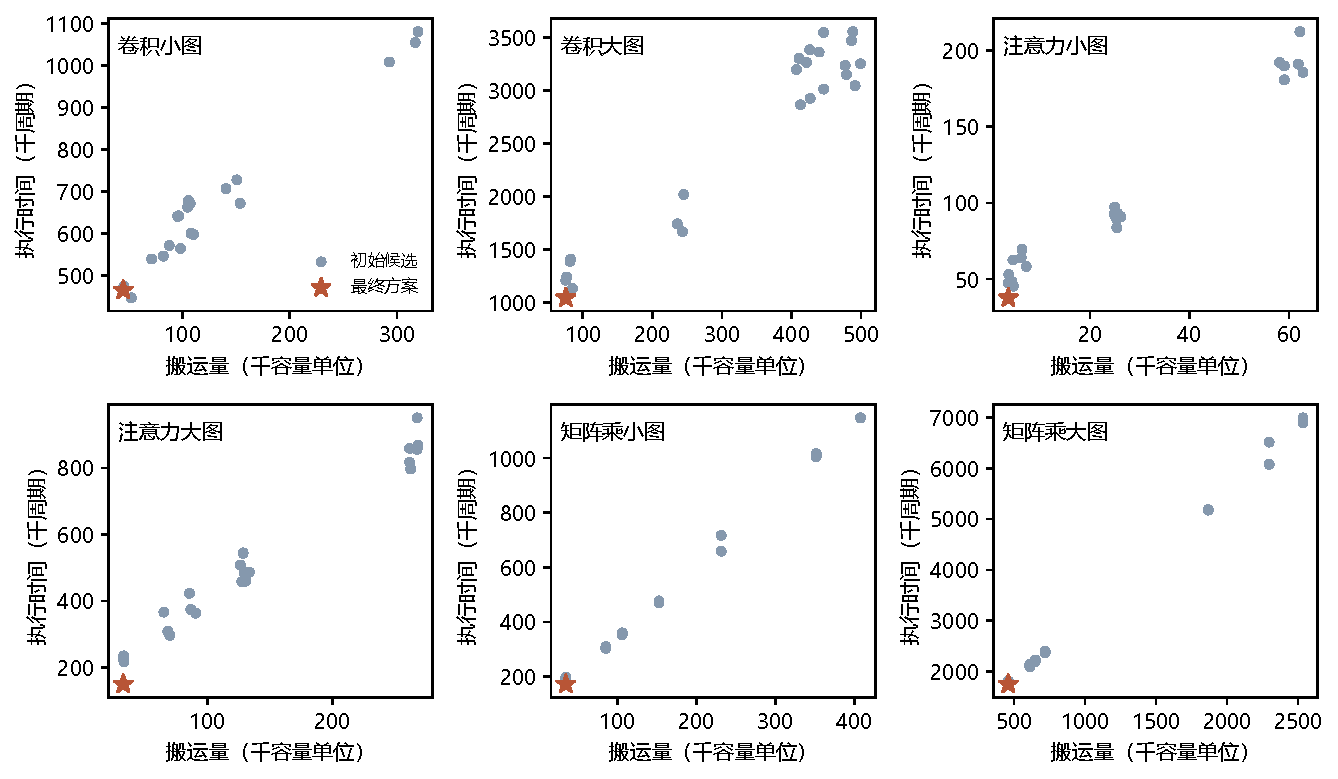
\includegraphics[width=\linewidth]{../figures/npu2025/tradeoff.pdf}
\caption{初始候选的时间与搬运量分布及最终方案}\label{fig:tradeoff}\end{figure}
图\ref{fig:tradeoff}表明，局部内存收益并不充分代表全图代价。先处理能释放大缓冲区的操作，可能同时启动更多尚不能结束的依赖分支，反而抬高后续驻留量。深度优先的前驱访问顺序也会改变共享数据的重用距离。故本研究的敏感性结论是规则选择依赖图结构，不能将某个参数称为普遍最优。六图均为同一题面提供的测试集，本轮没有额外的独立图集来验证泛化能力。

\subsection{手算例与反例校验}
构造两个无依赖操作，分别运行于输入和输出搬运单元，耗时为 10 和 20 周期，缓冲区大小均为 4。使用互不重叠的地址时，总时间为 20；复用同一地址时，释放到申请依赖使总时间为 30。该例同时检验跨单元并行与物理地址串行化，避免评价器错误地把整个调度序列串行执行或完全忽略复用等待。

对输入复制缓冲区插入一次换出，额外搬运量为 4；在测试给定的顺序及复用关系下，总时间为 188 周期。对非输入复制缓冲区执行相应测试，搬运量为 8，总时间为 346。二者分别覆盖零耗时换出与双向搬运公式。人为注入地址重叠、拓扑逆序、偏移越界和节点重复，检查程序均拒绝这些错误附件。

最终六图均检查全部原始依赖和新增换出节点、连续空间占用、使用时驻留以及执行单元互斥。下界取各执行单元总工作量与原图关键路径的最大值；由于未求解全局优化，该下界只用于合理性检查，不能证明候选最优。校验程序与求解器共享输入解析，仍可能存在共同的题意理解偏差，需要结合题面复核。

